\section{Simulations}
\label{sec:gamma}

In the final part of this exercise, a Monte Carlo technique is applied to the problem of a beam of unstable nuclei injected travelling towards a detector \SI{2}{\meter} away at \SI{2000}{\kilo\meter\per\second} with average lifetime \SI{520}{\micro\second}. The resolution of the detector is also modelled using Gaussian smearing.

\subsection{Decay Times}
\label{subsec:decay_times}

As this is a discrete event occurring a known average number of times in unit time interval, the radioactive decay of these nuclei can be modelled as a Poisson distribution. The average number of decays per second, $f$, is the reciprocal of the average lifetime, $\tau$, $f = \frac{1}{\tau}$. The decay times are then produced by generated a number of Poisson-distributed decays giving the number of decays in that second. These are inverted to find the lifetimes of the nuclei. As the nuclei are travelling at a constant speed of \SI{2000}{\kilo\meter\per\second}, the distance from the injection point at which the nuclei decay can be easily calculated using the equation $\text{decay position} = \text{lifetime} \times \text{speed}$. The distance travelling before the decay is thus also Poisson-distributed, with mean of \SI{1.04}{\meter}, as shown in Figure \ref{fig:decays}.

\begin{figure}
    \centering
    \includegraphics[width=\linewidth]{graphs/gamma/gamma_decays}
    \caption{Poisson-distributed decay times and positions.}
    \label{fig:decays}
\end{figure}

\subsection{Decay Angles}
\label{susbec:decay_angles}

Next the angles at which the emitted $\gamma$-rays decay need be calculated. Although it may seem intuitive, it is incorrect to choose both the azimuth, $\varphi$, and the altitude, $\theta$, to be evenly distributed. This is because the aim is to generate an area \textit{density} of angles, or an even number of angles in unit area; the area of a small area element of a sphere is given by\cite{WolframPointPicking}:
\begin{equation}
    \dd \Omega = \sin(\theta) \dd \varphi \dd \theta.
    \label{eqn:spherical_area_element}
\end{equation}

Hence, whilst $\varphi$ should be a uniformly distributed random number on interval $[0, 2\pi)$, $\theta$ should be sinusoidally distributed on interval $[0, pi]$. As calculated previously, $\varphi$ can be distributed sinusoidally by using the analytic inversion formula given in Equation \ref{eqn:analytic_sin_inverted}. In other words, if $u, v$ are random evenly distributed variables on $(0,1)$ as given by \texttt{numpy.random.random}:
\begin{align}
    \varphi &= 2\pi u, \\
    \theta  &= \arccos(2v - 1).
\end{align}

This effect of clumping at the poles when the points are picked incorrectly is shown in Figure \ref{fig:spheres}, taken as a snapshot of the interactive Mayavi visualisation accessible via the Python script \texttt{gamma/sphere\_mayavi.py}.

\begin{figure}
    \centering
    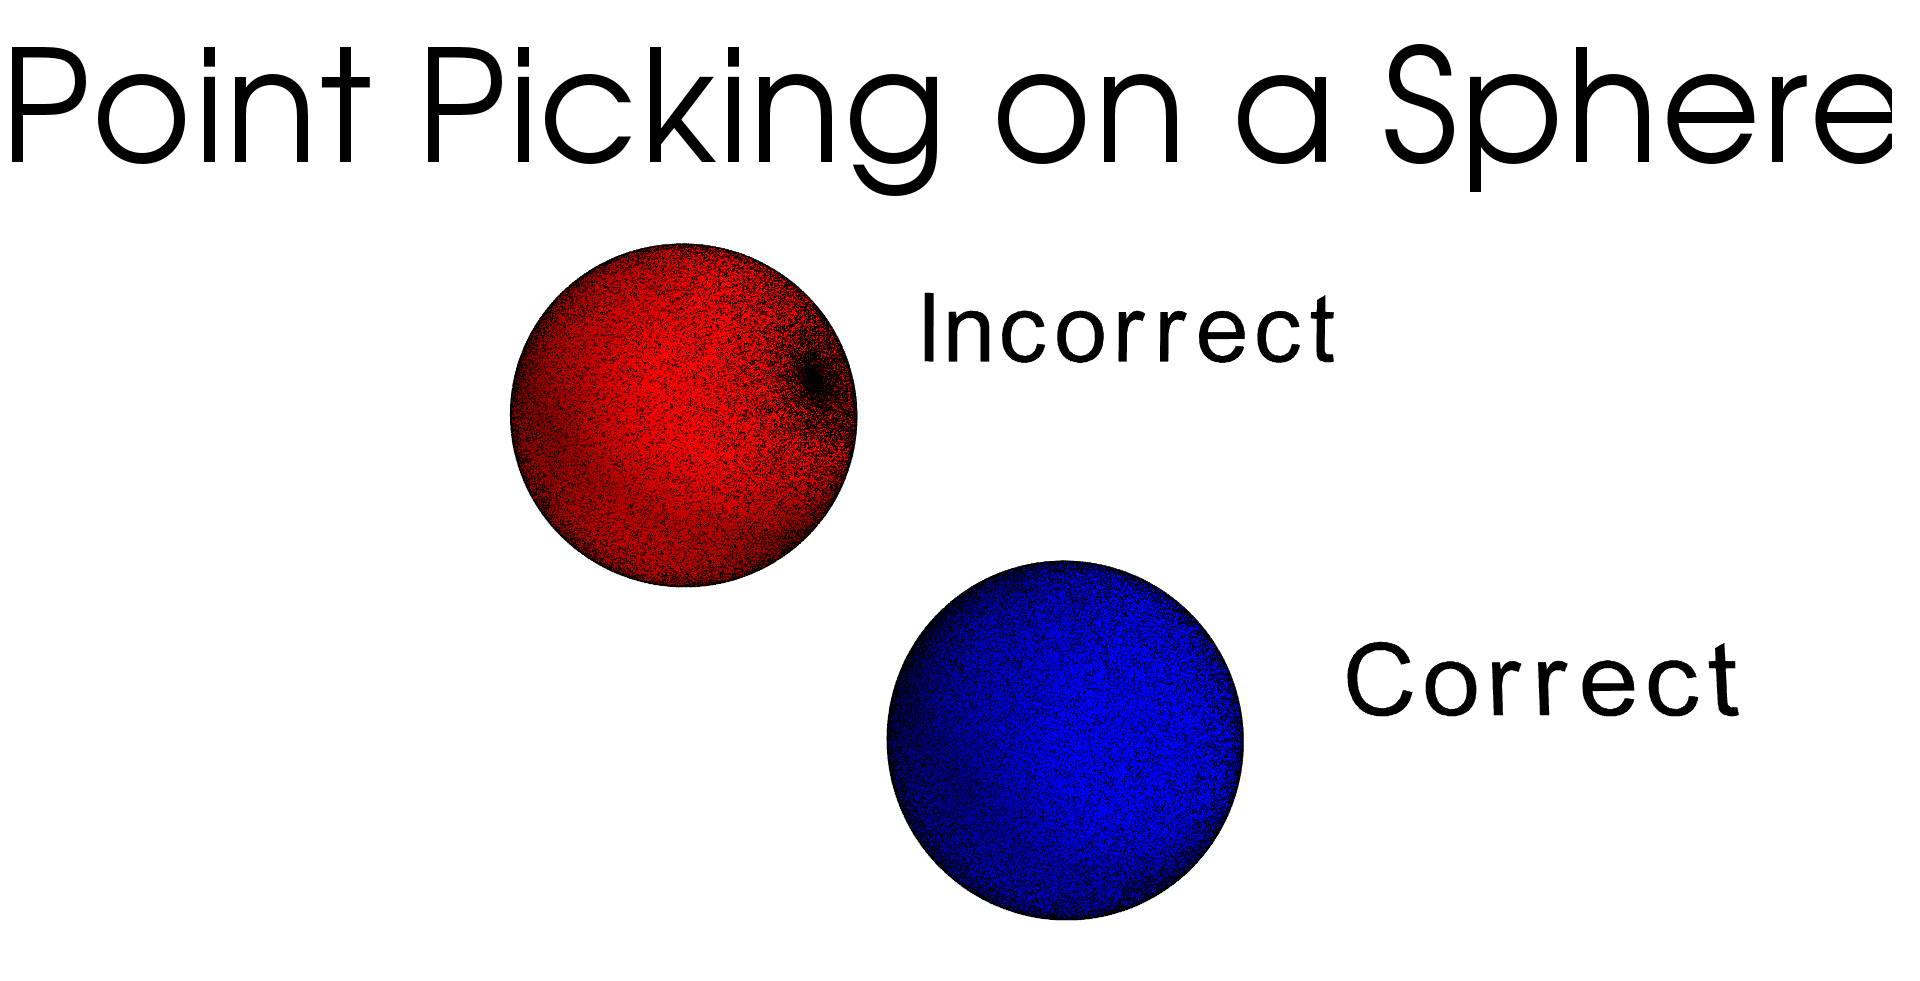
\includegraphics[width=\linewidth]{graphs/gamma/spheres}
    \caption{An illustration of the clumping that occurs when incorrectly picking points on a sphere. The black dots represent random points. Blue sphere shows correctly distributed points; red sphere shows incorrectly distributed points.}
    \label{fig:spheres}
\end{figure}

Now that the decay angles for the $\gamma$-ray have been correctly chosen so as to prevent clumping, all that need be done is to calculate the $X$ position and $Y$ position of the $\gamma$-rays when (or if) they intersect with the detector screen.

\subsection{Detector Reading Calculations}
\label{subsec:detector_reading_calculations}

The spherical coordinate system is set up such that $x$ points directly towards (perpendicular to) the detector, $y$ points parallel to the detector in the direction of $-X$ on the plane of the detector screen and $z$ points parallel to the plane of the detector in the $+Y$ direction on the plane of the detector screen. The standard equations for converting spherical coordinates to Cartesian are:
\begin{align}
    x &= r\cos(\varphi)\cos(\theta), \\
    y &= r\cos(\varphi)\sin(\theta), \\
    z &= r\sin(\varphi),
\end{align} where $r$ is the radial coordinate. To find the position the $\gamma$-ray hits the detector, $x$ is set to a constant, $d = $ distance from decay position to detector screen. Thus:
\begin{align}
    r &= \frac{d}{\cos(\varphi)\cos(\theta)} \notag \\
    \implies y &= d\tan(\theta) \label{eqn:gamma_y} \\
    \text{and}~z &= \frac{d\tan(\varphi)}{\cos(\theta)}. \label{eqn:gamma_z}
\end{align}

Note that these equations require $\varphi = 0$ to be pointing along the $x$-axis, so $\frac{\pi}{2}$ is taken from the sinusoidally distributed value of $\varphi$ so that this is the case.

Figure \ref{subfig:detector_unsmeared_nbins_200} shows the positions of the $\gamma$-rays as they hit the detector. This clearly shows a circular pattern on the centre of the detector screen, where most rays hit the centre of the screen, and fewer hit the edges. This is exactly what one would expect from Equations \ref{eqn:gamma_y} and \ref{eqn:gamma_z}, which essentially project the spherical envelope of randomly directional $\gamma$-rays onto the planar surface of the detector; at the centre of the screen the distance to the decay is minimal and the concentration of radiation is approximately the same as that in the small area pointing directly at the detector. In other words, map from spherical to planar surfaces has little effect. However, as the angles $\varphi$ and $\theta$ increase, the corresponding angle on the surface of the detector increases yet more so that changing $\varphi$ or $\theta$ a small amount causes a massive change in the position $(X,Y)$ on the detector.

\subsection{Detector Resolution}
\label{subsec:detector_resolution}

The detector being modelled is said to have $X$ and $Y$ resolutions of \SI{10}{\centi\metre} and \SI{30}{\centi\metre} respectively. One representation of this is to bin the $\gamma$-ray hit locations in bins of size \SI{10}{\centi\metre} by \SI{30}{\centi\metre}. This is shown in Figure \ref{subfig:detector_unsmeared}. The positions are still clearly circular contours of decreasing number of counts.

\begin{figure}
    \centering
    \subfloat[200 bins]{
        \includegraphics[width=\linewidth]{graphs/gamma/gamma_detector_unsmeared_200_bins}
        \label{subfig:detector_unsmeared_nbins_200}
    } \\
    \subfloat[Bins reflecting resolution]{
        \includegraphics[width=\linewidth]{graphs/gamma/gamma_detector_unsmeared}
        \label{subfig:detector_unsmeared}
    }
    \caption{2d histogram of positions of $\gamma$-rays as they hit the detector, first with 200 bins, showing the real distribution of $\gamma$-ray hit locations, and secondly with bins reflecting the resolution of the detector.}
    \label{fig:detector_unsmeared}
\end{figure}

In addition to this, the resolution of the detector, as a fundamental limiting factor to its ability to accurately record position data, is modelled by smearing the hit location data. This is done by adding a random normally distributed value to each hit location before binning, with mean equal to that hit location and standard deviation in $X$ and $Y$ directions equal to the resolution in that axis. The effect of this is to spread out the hits so that the counts at the centre are lowered, but the counts around the edges are increased. This is shown in Figure \ref{fig:detector_smeared}, which shows both the smeared locations with a large number of bins (Figure \ref{subfig:detector_smeared_nbins_200}), and with the bins reflecting the resolution (Figure \ref{subfig:detector_smeared}).

\begin{figure}
    \centering
    \subfloat[200 bins]{
        \includegraphics[width=\linewidth]{graphs/gamma/gamma_detector_smeared_200_bins}
        \label{subfig:detector_smeared_nbins_200}
    } \\
    \subfloat[Bins reflecting resolution]{
        \includegraphics[width=\linewidth]{graphs/gamma/gamma_detector_smeared}
        \label{subfig:detector_smeared}
    }
    \caption{2d histogram of positions of $\gamma$-rays as they hit the detector, after smearing, first with 200 bins, showing the real distribution of $\gamma$-ray hit locations, and secondly with bins reflecting the resolution of the detector.}
    \label{fig:detector_smeared}
\end{figure}

\subsection{Improvements}
\label{subsec:improvements}

There are several unaccounted for factors in this simulation that would improve the accuracy and realism of the simulation. For instance, real particle detectors have a dead time, meaning that there is a short period of time after a particle is detected that the detector cannot recognise any more signals in that area. Given the $\gamma$-rays in this simulation all travel at $c$, it would be possible to improve this simulation by calculating the time each particle hits the detector, and ignoring any hits a period $\tau$ after the detector recognises a signal. Silicon detectors also suffer from radiation damage, which in a limited sense could be modelled in this Monte Carlo simulation by introducing some random variables representing the changes to the characteristics of the detector and loss of hits due to the detector damage\cite{Moll99}.
